\documentclass{beamer}
\usepackage{amssymb}
\usepackage{xcolor}

% \usepackage{beamerthemesplit} // Activate for custom appearance

\title{Inefficiencies in the Unfettered Market \\ \large Perspectives on Economic Studies TA session}
\author{Qing Zhang}
\institute{Columbia University}
\date{\today}

\begin{document}
\frame{\titlepage}

\frame{
\frametitle{(In)efficiency of the Market}
\begin{itemize}
\item Are free markets Pareto efficient? Perhaps one of the most fundamental questions in economics. 
\item We have seen in undergraduate classes a laundry list of cases where there is inefficiency in the market: externalities, public goods, monopoly, etc...
\item Clearly, if an action that I choose directly enter the utility function of another individual (e.g., talking in a library), and I do not take that into account, the resulting equilibrium will generally not be efficient.  
\item Asymmetric information frequently gives rise to a subtler form of externality: individual choices collectively determine an aggregate variable (price, for example) which individuals fail to take into account.  
\item Greenwald-Stiglitz 1986 gives an elegant formula to determine the welfare impact of such externalities and taxes (subsidies) targeted at such externalities. They also provide many examples where asymmetric information problems are cast in this light.  
\end{itemize}

}

\frame{
\frametitle{Today}
\begin{itemize}
\item We are going to see two special cases of this framework: moral hazard and adverse selection in the insurance market. 
\item Papers we talk about:
\begin{itemize}
\item Arnott, Greenwald and Stiglitz, 1994, Information and Economic Efficiency 
\item Rothschild and Stiglitz, 1976, Equilibrium in Competitive Insurance Markets: An Essay on the Economics of Imperfect Information
\end{itemize}
\end{itemize}

}

\frame{
\frametitle{Today}
\begin{itemize}
\item A caveat: we will see from the models that we can establish inefficiencies in the market in a rigorous fashion, but there is a huge leap from the theory to making judgments about the desirability of real-world policies and institutions. 
\item In fact, one can argue that many problems today, especially those facing developing countries, stem from the fact that the market is missing in many situations, and individuals' choices are constrained by arbitrary restrictions imposed by the government. 
\item It goes without saying that government policies \textit{can} work does not imply that it is easy to determine optimal policies, or that governments do adopt optimal policies. Avoid black-and-white stances on the desirability of interventions v. free market. 
\end{itemize}
}

\frame{
\frametitle{Arnott, Greenwald and Stiglitz 1994\\\large Main Idea}
\begin{itemize}
\item If individuals exert more effort to avoid accidents, the market insurance premium will go down, which benefits all individuals. This is an externality that they do not take into account. 
\item Government policies that taxes commodities that are substitutes to effort and/or subsidizes commodities that are complements to effort will induce more effort, and result in welfare gains that outweigh the dead-weight losses induced by the tax/subsidy. 
\item An application of Greenwald-Stiglitz.
\end{itemize}
}


\frame
{
  \frametitle{Taxation under Moral Hazard}
\begin{itemize}
\item Express individual's indirect utility function as $V(\alpha, \beta, e)$. 
\begin{itemize}
\item $\alpha$: net benefit when there is an accident. Higher $\alpha$ represents higher coverage of risk.
\item $\beta$: premium.
\item $e$: effort level, can either be high $e^H$ or low $e^L$. 
\end{itemize}
\item In the event of accident, income will be $y-d+\alpha$. In the event of no accident, income will be $y-\beta$.
\item Probability of accident $p^H = p(e^H)$, $p^L = p(e^L)$, $p^H<p^L$.
\end{itemize}

 }
 
\frame{   
\frametitle{Taxation under Moral Hazard}
\begin{itemize}
\item Solve for optimal tax rate under the constraint that it is impossible to monitor effort, and therefore it has to be in the individual's private interest to exert hight effort. 
\item max $V^H(\alpha, \beta, q)$ \\ \vspace{10pt} s.t. $\alpha p^H = \beta (1-p^H) + (q-1) X^H$ \\ \vspace{5pt} \hspace{15pt} $V^H(\alpha, \beta, q) > V^L(\alpha, \beta, q)$
\end{itemize}
 
 }
 
\frame{
\frametitle{Taxation under Moral Hazard}
\begin{itemize}
\item Lagrangian 
\begin{align*}
\mathcal{L} = V^H + \gamma(\alpha p^H - \beta (1-p^H) - (q-1) X^H)\\ + \lambda (V^H(\alpha, \beta, q) - V^L(\alpha, \beta, q))  
\end{align*}

\item Differentiate the Lagrangian with respect to $q$, $\alpha$ and $\beta$:
\begin{align}
\frac{\partial \mathcal{L}}{\partial q_k} &= V^H_k - \gamma X^H_k + \lambda (V^H_k - V^L_k) \\
\frac{\partial \mathcal{L}}{\partial \alpha} &= V^H_\alpha + \gamma p^H + \lambda(V^H_\alpha - V^L_\alpha) = 0 \\
\frac{\partial \mathcal{L}}{\partial \beta} &=  V^H_\beta - \gamma (1-p^H) + \lambda(V^H_\beta - V^L_\beta) = 0
\end{align}
\item If $\frac{\partial \mathcal{L}}{\partial q_k} \neq 0$ at $q_k=1$, the optimal tax is not zero. Can think of good $k$ as cigarette here for concreteness. 
\end{itemize}
 
 }
 
\frame{
\frametitle{Taxation under Moral Hazard}
\begin{itemize}
\item Recall Roy's Identity 
\[\frac{\partial v(p, y)}{\partial p_k} = -x_k(p, y)\frac{\partial v(p,y)}{\partial y}\]
Effect of a price increase of good $k$ on utility is equal to (negative) consumption of good $k$ times the effect of income increase on utility.
\item Apply Roy's Identity here: 
\[V^H_k = - p^H\mu^{H1}X^{H1}_k - (1-p^H)\mu^{H0}X^{H0}_k\]
\item $\mu$ is marginal effect of income. Notice the double super-script here: $H1$ represents when effort is high and there is an accident, etc. 
\item Also easy to see 
\[V^H_\alpha = p^H \mu^{H1}, V^H_{\beta} = -(1-p^H)\mu^{H0}\]
\item Notice that this implies 
\[V^H_k + X^{H1}_k V^H_\alpha - X^{H0}_k V^H_{\beta} = 0\]
\end{itemize}

} 
 
\frame{
\frametitle{Taxation under Moral Hazard}
\begin{itemize}
\item Use this equation to cancel terms
\begin{align}
\frac{\partial \mathcal{L}}{\partial q_k} &= \textcolor{blue}{V^H_k} - \gamma \textcolor{red}{X^H_k} + \lambda (\textcolor{blue}{V^H_k} - V^L_k) \\
\frac{\partial \mathcal{L}}{\partial \alpha} &= \textcolor{blue}{V^H_\alpha} + \gamma \textcolor{red}{p^H} + \lambda(\textcolor{blue}{V^H_\alpha} - V^L_\alpha) = 0 \\
\frac{\partial \mathcal{L}}{\partial \beta} &=  \textcolor{blue}{V^H_\beta} - \gamma \textcolor{red}{(1-p^H)} + \lambda(\textcolor{blue}{V^H_\beta} - V^L_\beta) = 0
\end{align}
\item (4) + (5) * $X^{H1}_k$ -(6) * $X^{H0}_k$ $\implies$ The blue terms cancel out among themselves. So do the red terms. There remains:
\[\frac{\partial \mathcal{L}}{\partial q_k} = \lambda (p^L\mu^{L1}(X^{L1}_k - X^{H1}_k) + (1-p^L)\mu^{L0}(X^{L0}_k - X^{H0}_k))\]
\end{itemize}
} 
 
\frame{
\frametitle{Taxation under Moral Hazard}
\begin{itemize}
\item If consumption of cigarettes does not depend on effort, i.e., $X^{L1}_k = X^{H1}_k$ and $X^{L0}_k = X^{H0}_k$. Then $\frac{\partial \mathcal{L}}{\partial q_k}|_{q=1} = 0$. Optimal tax is zero.
\item However, if cigarettes and effort are substitutes (e.g., smoking makes it more costly to stay healthy), $X^{L1}_k > X^{H1}_k$ and $X^{L0}_k > X^{H0}_k$. Then $\frac{\partial \mathcal{L}}{\partial q_k}|_{q=1} > 0$. Optimal tax on cigarettes is positive. 
\item Intuition: tax introduces a deadweight loss by changing consumption levels, but that loss is second-order.
\begin{itemize}
\item In choosing consumption, the individual is maximizing utility and satisfying his FOC. Therefore if we Taylor-expand his utility function around his optimal consumption choice, the linear terms of consumption drop out. 
\item But when we induce the individual to exert more effort, the government's budget constraint is relaxed, which can be understood as resulting in either a reduction in the premium ($\beta$) or more coverage ($\alpha$). This has a first-order effect on $V(\alpha, \beta, q, e)$, because the individual (as a price taker) does not optimize w. r. t. $\alpha$ or $\beta$.    
\end{itemize}
\end{itemize}
} 

\frame{
\frametitle{Rothschild and Stiglitz 1976 \\\large Main Idea}
\begin{itemize}
\item In the presence of information asymmetry, a competitive equilibrium may not exist.
\item Even when an equilibrium exists, it is not efficient (everyone will be made better off if only people would tell the truth about their types). 
\item The equilibrium may not even be constrained efficient (that is, given constraints imposed by information asymmetry, there may be ways to effect a Pareto improvement.)
\end{itemize}
} 

\frame{
\frametitle{Adverse Selection in a Competitive Insurance Market}
\begin{itemize}
\item Probability of accident: $p$
\item Wealth under no accident: $W_1 = W$. Wealth under accident: $W_2 = W-d$
\item Insurance contract $\alpha = (\alpha_1, \alpha_2)$, such that under the contract, $W_1 = W - \alpha_1, W_2 = W-d+\alpha_2$
\item (Risk-averse) buyer can choose only one insurance contract. Maximizes expected utility
\[(1-p)U(W_1) + pU(W_2)\] 
\item Insurance company designs which contracts to offer. Maximizes expected profit
\[(1-p)\alpha_1 - p\alpha_2\]
\end{itemize}

}

\frame{
\frametitle{Adverse Selection in a Competitive Insurance Market}
\begin{itemize}
\item An equilibrium is a set of contracts such that
\begin{itemize}
\item No contract in the equilibrium set makes negative expected profit.
\item  there is no contract outside the equilibrium set that, if offered, will make a nonnegative profit.
\item Notice the role of competition here.
\end{itemize}
\item Two classes of customers: high-risk individuals with $p^H$ and low-risk individuals with $p^L$. \\
\item Now we establish the following in order:
\begin{itemize}
\item There cannot be a pooling equilibrium.
\item If there is a separating equilibrium, it must be of a particular form. 
\item Such an equilibrium may not exist.
\end{itemize}
\end{itemize}

}

\frame{
\frametitle{No Pooling Equilibrium}
\begin{figure}
\centering
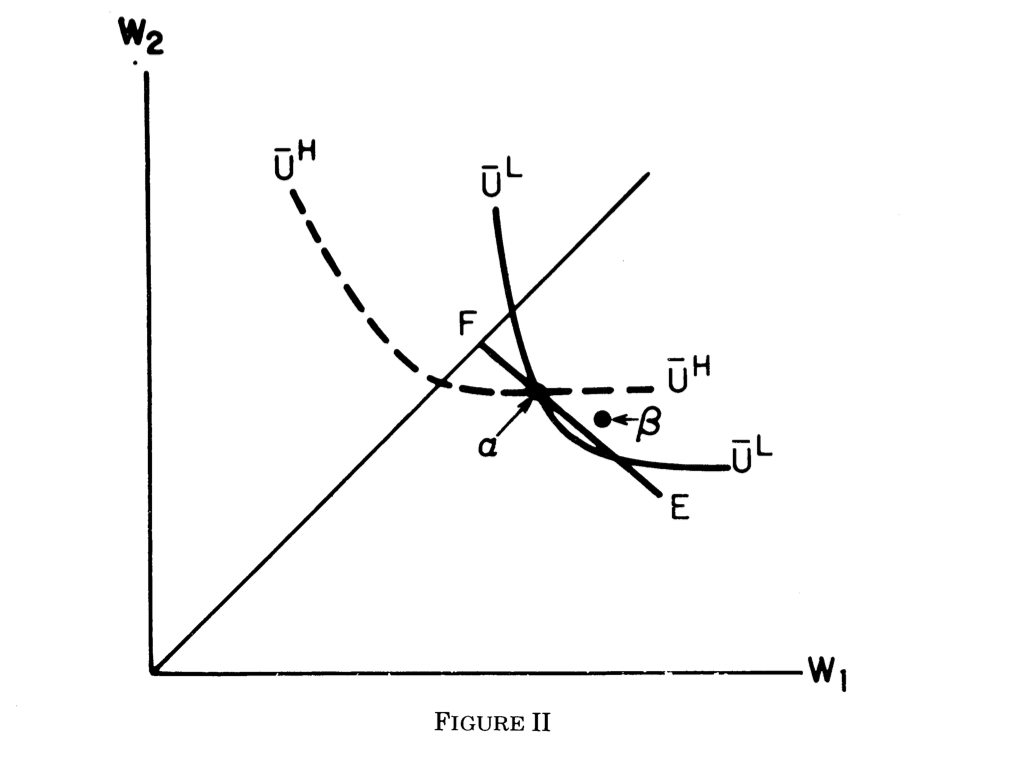
\includegraphics[width=0.68\textwidth]{nopooling}
\end{figure}
\begin{itemize}
\item Suppose $\alpha$ is a pooling equilibrium. Then it is possible to find a contract $\beta$ that will attract the low-risks, and make a positive profit. This violates our definition of equilibrium. 
\end{itemize}

}

\frame{
\frametitle{(Candidate) Separating Equilibrium}
\begin{figure}
\centering
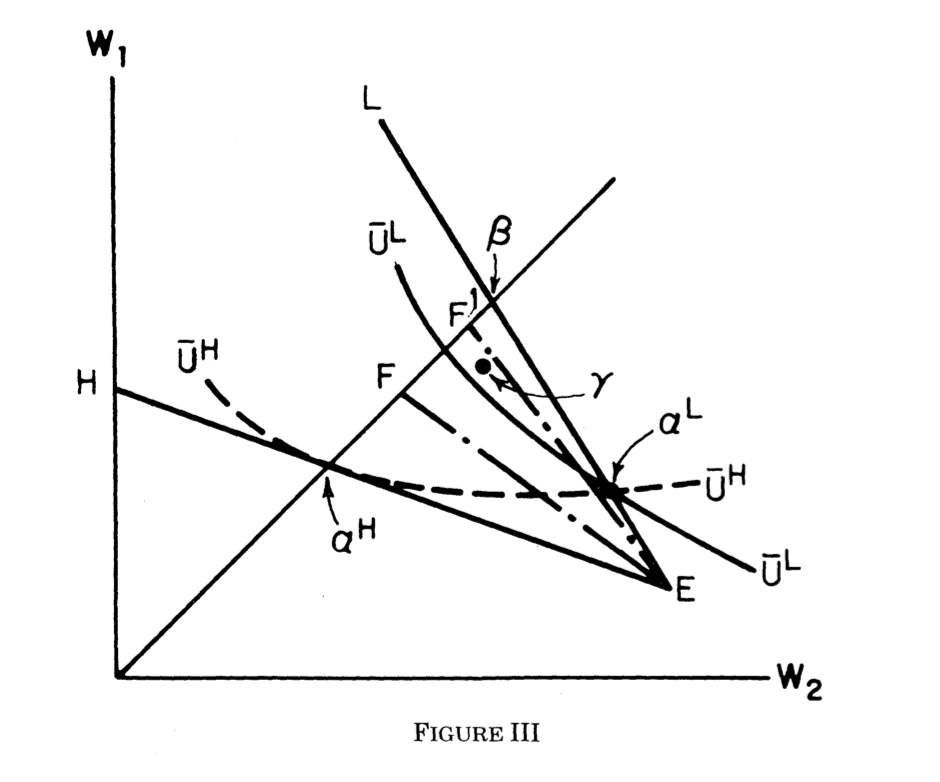
\includegraphics[width=0.5\textwidth]{separating}
\end{figure}
\begin{itemize}
\item There can only exist one separating equilibrium: $\{\alpha^H, \alpha^L\}$
\item The key is a self-selection constraint: insurance offered to low-risks must be sufficiently unattractive to the high-risks lest they pool with the low-risks.
\item As a result, the low-risks are not fully insured. If $\beta$ is offered, the high-risks will pool, and $\beta$ will make a negative profit. 
\end{itemize}
}

\frame{
\frametitle{An Equilibrium May not Exist}
\begin{figure}
\centering
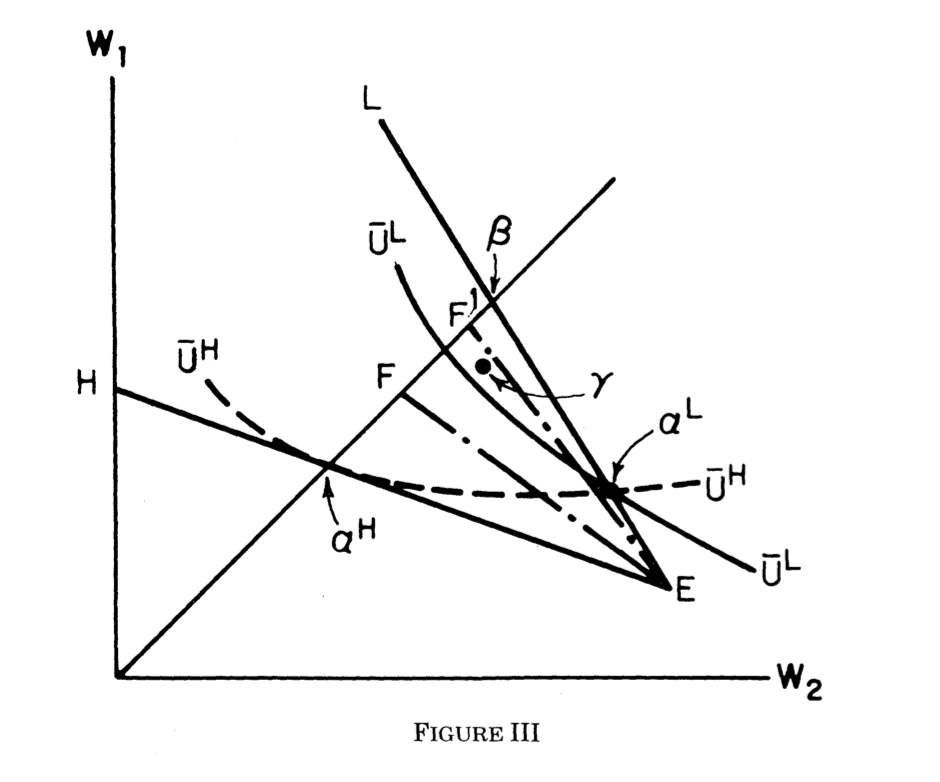
\includegraphics[width=0.5\textwidth]{separating}
\end{figure}
\begin{itemize}
\item If the high-risks are relatively few, there exists a contract $\gamma$ that both types will prefer, and that makes a positive profit. 
\item This upsets the separating equilibrium. 
\end{itemize}
}

\frame{
\frametitle{Cross-Subsidization}
\begin{itemize}
\item If we relax the assumption that each insurance contract has to individually break even, we can design contracts where the low-risks subsidize the high-risks and effect a Pareto improvement.
\item The high-risks will always be fully insured. We maximize welfare of the low-risks subject to the self-selection constraint. 
\item Let the high-risks receive subsidy $a$ from low-risks in both states of world. This reduces income of low-risks by $\gamma a$ ($\gamma = \lambda/(1-\lambda)$, ratio of number of two types). 
\end{itemize}
}

\frame{
\frametitle{Cross-Subsidization}
\begin{itemize}
\item Income of high-risks in both states will be
\[Y = W - p^Hd + a\] 
\item Income of low-risks under no accident
\[X = W_0 - \gamma a - \alpha_2p^L/(1-p^L)\]
\item Income of low-risks under accident
\[Z = W_0 - d - \gamma a + \alpha_2\]
\item Choose $a$ and $\alpha_2$ to maximize
\[U(X)(1-p^L) + U(Z)p^L\]
subject to 
\begin{align*}
U(Y) &\geq U(X)(1-p^H) + U(Z)p^H\\
a &\geq 0
\end{align*}
\end{itemize}
}

\end{document}

